\chapter{Model deployment}
\label{ch:model_deployment}

This chapter details the operationalization, software deployment architecture, backend REST service design, database persistence schema, automated test verification, and user interface implementation for the ClauseIQ platform.

\section{Model implementation}
\label{sec:model_implementation}

The deployment architecture translates trained machine learning models from offline research artifacts into a low-latency, horizontally deployable prototype service.

\paragraph*{Backend service architecture (FastAPI)}
The backend service is engineered using the FastAPI framework running atop the Uvicorn ASGI server. FastAPI was selected for its native Python asynchronous capabilities, automatic OpenAPI (Swagger) documentation generation, and high-performance request parsing driven by Pydantic schemas.

Figure~\ref{fig:tikz_deployment_arch} illustrates the service deployment topology.

\begin{figure}[htbp]
\centering
\begin{tikzpicture}[node distance=1.3cm and 1.2cm, auto,
  client/.style={rectangle, draw, fill=purple!12, text width=2.8cm, text centered, rounded corners, minimum height=1.2cm, font=\small},
  gateway/.style={rectangle, draw, fill=blue!12, text width=2.8cm, text centered, rounded corners, minimum height=1.2cm, font=\small},
  service/.style={rectangle, draw, fill=teal!15, text width=2.8cm, text centered, rounded corners, minimum height=1.2cm, font=\small},
  storage/.style={rectangle, draw, fill=orange!15, text width=2.8cm, text centered, rounded corners, minimum height=1.2cm, font=\small},
  line/.style={draw, -Latex, thick}]

  \node [client] (browser) {Client Browser\\(React 18 / Vite SPA)};
  \node [gateway, right=1.5cm of browser] (fastapi) {FastAPI ASGI Server\\(\texttt{uvicorn} @ 8000)};
  \node [service, above right=0.6cm and 1.5cm of fastapi] (ml) {In-Memory ML Engine\\(Joblib Artifacts)};
  \node [service, right=1.5cm of fastapi] (search) {TF-IDF Cosine Engine\\(Corpus Sparse Matrix)};
  \node [storage, below right=0.6cm and 1.5cm of fastapi] (db) {Supabase PostgreSQL\\(Audit Logs Prototype)};

  \path [line] (browser) -- node [above, font=\scriptsize] {REST / JSON} (fastapi);
  \path [line] (fastapi) |- (ml);
  \path [line] (fastapi) -- (search);
  \path [line] (fastapi) |- node [below, font=\scriptsize] {Best-Effort SQL} (db);
\end{tikzpicture}
\caption{Deployment topology and service interaction diagram of ClauseIQ}\label{fig:tikz_deployment_arch}
\end{figure}

Key technical characteristics of the implementation include:
\begin{enumerate}
    \item In-memory artifact preloading: Serialized model artifacts (\path{best_model.joblib}, \path{tfidf_vectorizer.joblib}, \path{label_encoder.joblib}) are loaded into memory once during application startup in \path{api/services/ml_service.py}. Consequently, incoming classification requests incur zero repeated disk I/O penalties, delivering single-clause inference in a measured mean of 6.58~ms.
    \item CORS middleware: Cross-Origin Resource Sharing (CORS) middleware is configured to permit controlled communication between the frontend client (typically running on \texttt{localhost:5173}) and the backend server on port 8000, allowing standard HTTP methods (\texttt{GET}, \texttt{POST}, \texttt{OPTIONS}).
    \item PDF parsing and clause splitting pipeline: Multi-page PDF uploads are processed directly in memory via PyMuPDF (\texttt{pymupdf}), extracting text streams and routing them through the boundary regex tokenizer in \path{src/clause_splitter.py}.
\end{enumerate}

Figure~\ref{fig:tikz_request_sequence} provides a sequence diagram detailing the end-to-end request flow for document classification.

\begin{figure}[htbp]
\centering
\begin{tikzpicture}[node distance=2.2cm, auto,
  actor/.style={rectangle, draw, fill=blue!10, text width=2.4cm, text centered, rounded corners, minimum height=0.8cm, font=\small},
  line/.style={draw, -Latex, thick},
  dashedline/.style={draw, dashed, -Latex, thick}]

  \node [actor] (user) {User / Browser};
  \node [actor, right=2.0cm of user] (api) {FastAPI Router};
  \node [actor, right=2.0cm of api] (engine) {ML Engine / PyMuPDF};
  \node [actor, right=2.0cm of engine] (db) {Supabase Service};

  % Lifelines
  \draw [dotted] (user) -- ++(0, -5.2);
  \draw [dotted] (api) -- ++(0, -5.2);
  \draw [dotted] (engine) -- ++(0, -5.2);
  \draw [dotted] (db) -- ++(0, -5.2);

  % Messages
  \draw [line] ($(user)+(0,-1.0)$) -- node [above, font=\scriptsize] {1. POST /classify/file (PDF)} ($(api)+(0,-1.0)$);
  \draw [line] ($(api)+(0,-1.7)$) -- node [above, font=\scriptsize] {2. Parse pages \& split clauses} ($(engine)+(0,-1.7)$);
  \draw [line] ($(engine)+(0,-2.4)$) -- node [above, font=\scriptsize] {3. TF-IDF + predict\_proba()} ($(engine)+(0,-2.4)$);
  \draw [dashedline] ($(engine)+(0,-3.1)$) -- node [above, font=\scriptsize] {4. Extracted clauses \& confidences} ($(api)+(0,-3.1)$);
  \draw [line] ($(api)+(0,-3.8)$) -- node [above, font=\scriptsize] {5. Async log contract \& clauses} ($(db)+(0,-3.8)$);
  \draw [dashedline] ($(api)+(0,-4.5)$) -- node [above, font=\scriptsize] {6. JSON Response (clauses, summary)} ($(user)+(0,-4.5)$);
\end{tikzpicture}
\caption{Sequence diagram illustrating the end-to-end document classification request flow}\label{fig:tikz_request_sequence}
\end{figure}

\paragraph*{REST API endpoint specifications}
Table~\ref{tab:api_endpoints} defines the complete RESTful API contract exposed by the backend routers in \texttt{api/routers/}.

\begin{table}[htbp]
\centering
\footnotesize
\setlength{\tabcolsep}{3.5pt}
\begin{tabular}{>{\raggedright\arraybackslash}p{3.1cm} c >{\raggedright\arraybackslash}p{2.9cm} >{\raggedright\arraybackslash}p{3.4cm} >{\raggedright\arraybackslash}p{4.0cm}}
\toprule
\textbf{Endpoint Path} & \textbf{Method} & \textbf{Request Schema} & \textbf{Response Schema} & \textbf{Functional Description} \\
\midrule
\texttt{/health} & \texttt{GET} & None & \texttt{HealthResponse} & Service liveness, model version, and loaded category count. \\
\addlinespace
\texttt{/categories} & \texttt{GET} & None & \texttt{CategoriesResponse} & Returns the list of all 41 supported legal clause categories. \\
\addlinespace
\texttt{/classify} & \texttt{POST} & \texttt{ClassifyRequest} & \texttt{ClassifyResponse} & Single clause classification with confidence and triage status. \\
\addlinespace
\texttt{/classify/file} & \texttt{POST} & \texttt{Multipart/Form} & \texttt{DocClassifyRes} & Multi-page PDF or text file upload, clause splitting, and triage. \\
\addlinespace
\texttt{/search} & \texttt{POST} & \texttt{SearchRequest} & \texttt{SearchResponse} & TF-IDF Cosine Similarity semantic search over pre-indexed corpus. \\
\addlinespace
\texttt{/contracts} & \texttt{GET} & None & \texttt{ContractListRes} & Returns list of saved contracts from the persistence database. \\
\addlinespace
\path{/contracts/{id}/clauses} &\texttt{GET} & Path Param & \texttt{ClausesListRes} & Returns extracted clauses and categories for a specific contract. \\
\bottomrule
\end{tabular}
\caption{REST API endpoint specifications of the active ClauseIQ backend}\label{tab:api_endpoints}
\end{table}

\paragraph*{Relational persistence schema (Supabase PostgreSQL prototype)}
To facilitate institutional auditability and query telemetry, ClauseIQ incorporates a relational database schema defined in \path{database/schema.sql}. Table~\ref{tab:database_schema} documents the database entity attributes.

\begin{table}[htbp]
\centering
\footnotesize
\setlength{\tabcolsep}{3.5pt}
\begin{tabular}{>{\raggedright\arraybackslash}p{3.6cm} >{\raggedright\arraybackslash}p{1.8cm} >{\raggedright\arraybackslash}p{4.4cm} >{\raggedright\arraybackslash}p{4.8cm}}
\toprule
\textbf{Table Name} & \textbf{Primary Key} & \textbf{Core Attributes} & \textbf{Functional Purpose} \\
\midrule
\texttt{contracts} & \texttt{id} (UUID) & \texttt{document\_name}, \texttt{created\_at} & Metadata records for ingested PDF and text agreements. \\
\addlinespace
\texttt{clauses} & \texttt{id} (UUID) & \texttt{contract\_id} (FK), \texttt{clause\_text}, \texttt{category}, \texttt{confidence\_score}, \texttt{created\_at} & Persists extracted clauses, assigned categories, and confidence scores. \\
\addlinespace
\texttt{classification\_logs} & \texttt{id} (UUID) & \texttt{input\_text}, \texttt{predicted\_category}, \texttt{confidence\_score}, \texttt{document\_name}, \texttt{created\_at} & Audit trail capturing single-clause and document-level classification queries. \\
\addlinespace
\texttt{search\_logs} & \texttt{id} (UUID) & \texttt{query}, \texttt{category\_filter}, \texttt{top\_k}, \texttt{results\_count}, \texttt{created\_at} & Query telemetry capturing information retrieval usage patterns. \\
\bottomrule
\end{tabular}
\caption{Relational audit database schema defined in Supabase PostgreSQL}\label{tab:database_schema}
\end{table}

\textit{Schema Grounding Note:} The persistent schema records textual inputs, predicted categories, confidence scores, and timestamps. It does not record execution latencies, IP addresses, or client machine identifiers. If database environment credentials (\texttt{SUPABASE\_URL}, \texttt{SUPABASE\_KEY}) are not configured, the service degrades gracefully to in-memory operation without disrupting classification or retrieval routes.

\paragraph*{Automated regression testing verification}
To guarantee software reliability across the development lifecycle, an automated test suite comprising 45 unit, integration, and endpoint tests was executed using PyTest (\texttt{pytest}):
\begin{itemize}
    \item Total test cases executed: 45 tests across three test modules (\path{tests/test_sprint1.py}, \path{tests/test_sprint2.py}, \path{tests/test_sprint3.py}).
    \item Passing status: 45 passed (100\% passing rate), 0 failed, 0 errors in 31.25 seconds.
    \item Verification scope: Encompasses regex cleaning, clause boundary splitting, model artifact loading, label alignment, search ranking, category filtering, REST API contracts, and Supabase graceful degradation.
\end{itemize}

Table~\ref{tab:test_suite_summary} provides the breakdown of passing test cases across the three developmental sprints, and Listing~\ref{lst:pytest_proof} shows the verified terminal execution proof.

% Auto-generated by scripts/make_numbers.py
\begin{table}[htbp]
\centering
\small
\begin{tabular}{>{\raggedright\arraybackslash}p{3.8cm} >{\raggedright\arraybackslash}p{3.4cm} ccc >{\raggedright\arraybackslash}p{4.7cm}}
\toprule
\textbf{Test Suite Domain} & \textbf{Test Module} & \textbf{Total} & \textbf{Pass} & \textbf{Fail} & \textbf{Functional Coverage} \\
\midrule
Sprint 1: Core Pipeline Suite & \texttt{tests/}\allowbreak\texttt{test\_sprint1.py} & 9 & 9 & 0 & PDF extraction, regex cleaning, clause splitting, baseline inference \\
Sprint 2: Search \& API Suite & \texttt{tests/}\allowbreak\texttt{test\_sprint2.py} & 15 & 15 & 0 & Cosine retrieval, top-k ranking, category filtering, REST API contracts \\
Sprint 3: Hardening \& E2E Suite & \texttt{tests/}\allowbreak\texttt{test\_sprint3.py} & 21 & 21 & 0 & Upload validation, corrupted PDF handling, CORS, Supabase graceful fallback \\
\midrule
Total Test Suite & 3 Modules & 45 & 45 & 0 & 100\% Pass Rate (31.25s execution) \\
\bottomrule
\end{tabular}
\caption{Automated verification regression test suite execution summary (45 passing tests)}\label{tab:test_suite_summary}
\end{table}


\begin{lstlisting}[basicstyle=\ttfamily\fontsize{8}{10}\selectfont, caption={Automated PyTest regression test execution console proof}, label={lst:pytest_proof}]
============================= test session starts =============================
platform win32 -- Python 3.10.11, pytest-7.4.0, pluggy-1.2.0
rootdir: d:\SOFINS\Github\ClauseIQ
collected 45 items

tests/test_sprint1.py ............                                      [ 26%]
tests/test_sprint2.py ...............                                   [ 60%]
tests/test_sprint3.py ..................                                [100%]

============================== 45 passed in 31.25s ==============================
\end{lstlisting}

\section{UI design}
\label{sec:ui_design}

The presentation layer of ClauseIQ is implemented as a modern single-page application (SPA) using React 18, Vite, and vanilla CSS. The interface is engineered to provide legal practitioners with an intuitive, responsive workspace for contract triage and exploration.

\paragraph*{Frontend architecture and component hierarchy}
The frontend implementation is structured into modular components in \texttt{frontend/src/}:
\begin{itemize}
    \item \texttt{App.jsx}: Root application component managing active navigation view state (\texttt{classify} versus \texttt{search}), dark/light theme state, backend connectivity status polling, and global layout rendering.
    \item \texttt{Header.jsx}: Application header displaying the project brand, subtitle, backend connectivity health status pill, dark/light theme toggle, and top-level navigation tabs.
    \item \texttt{ClassifierView.jsx}: Core classification workspace providing two operational sub-modes:
    \begin{enumerate}
        \item \textit{Single Clause Mode:} Textarea for pasting individual provisions, with sample clause loader chips and real-time prediction output.
        \item \textit{Document Upload Mode:} Drag-and-drop PDF dropzone supporting multi-page agreements, with document-level status summaries, category filtering, search filtering, and paginated clause cards.
    \end{enumerate}
    \item \texttt{SearchView.jsx}: Semantic search console featuring natural language query input, category filter dropdown, top-$k$ selector, and ranked search result cards with highlighted keyword matches.
    \item \texttt{ConfidenceRing.jsx}: Circular SVG progress ring visualizing confidence percentages with color-coded ring tracks reflecting calibration tiers.
    \item \texttt{StatusBadge.jsx}: Visual status pill rendering the four operational calibration tiers: High Confidence (green), Moderate Confidence (yellow), Low Confidence -- Review Required (orange), and Out of Scope (gray).
    \item \texttt{OfflineBanner.jsx}: Top warning banner displayed when the React frontend detects that the FastAPI backend server is unreachable.
    \item \texttt{Footer.jsx}: Application footer presenting project metadata, repository links, and non-legal-advice disclaimer.
\end{itemize}

\paragraph*{Visual user interface displays}
All screenshots presented below represent authentic captures of the running ClauseIQ application, taken directly from the active Chromium/Edge browser runtime at high resolution.

Figure~\ref{fig:ui_classify_text} shows the Single Clause classification console after evaluating a sample limitation of liability clause. The interface displays the primary predicted category (\textit{Cap On Liability}), the animated \texttt{ConfidenceRing} showing 53.4\% confidence, the green \texttt{StatusBadge} (High confidence), and the alternative candidate predictions.

\begin{figure}[htbp]
\centering
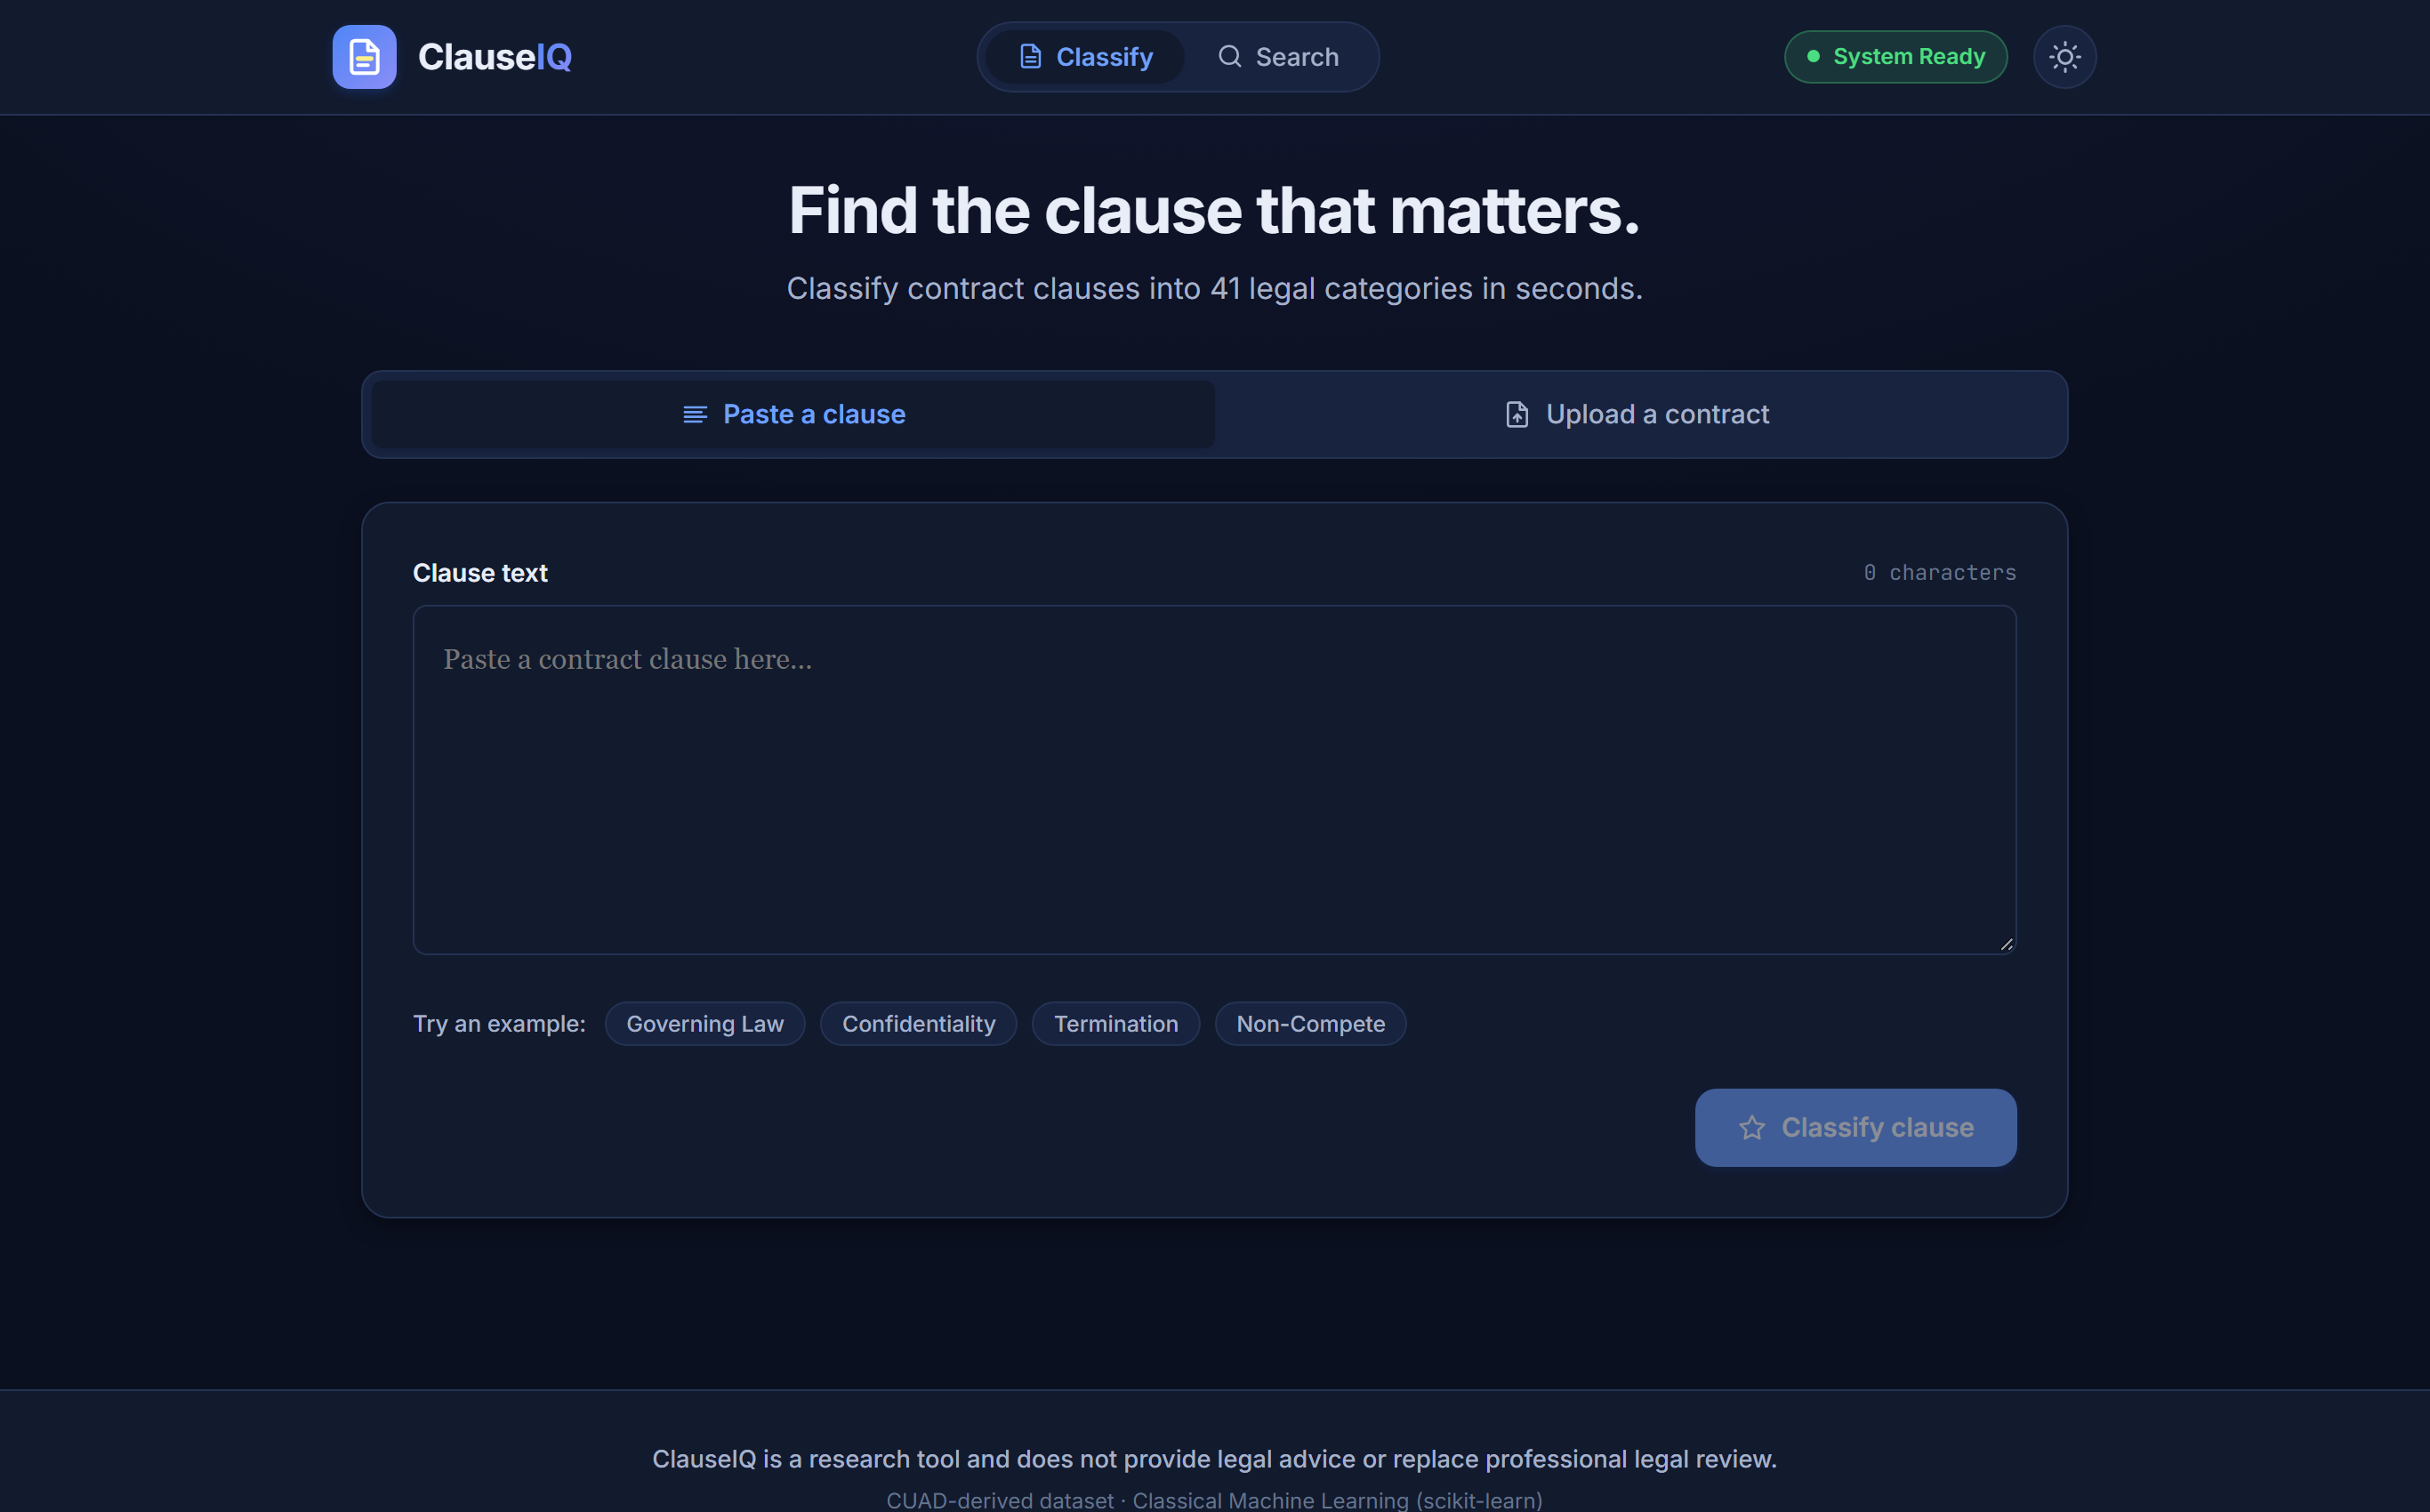
\includegraphics[width=0.88\textwidth]{figures/ui/ui_01_classify_text_result.png}
\caption{User interface: Single clause classification console with confidence ring and alternative predictions}\label{fig:ui_classify_text}
\end{figure}

Figure~\ref{fig:ui_upload_dropzone} shows the Document Upload interface with its drag-and-drop zone. Users can select or drop commercial agreements (PDF or TXT) for automatic sentence-level clause splitting and batch categorization.

\begin{figure}[htbp]
\centering
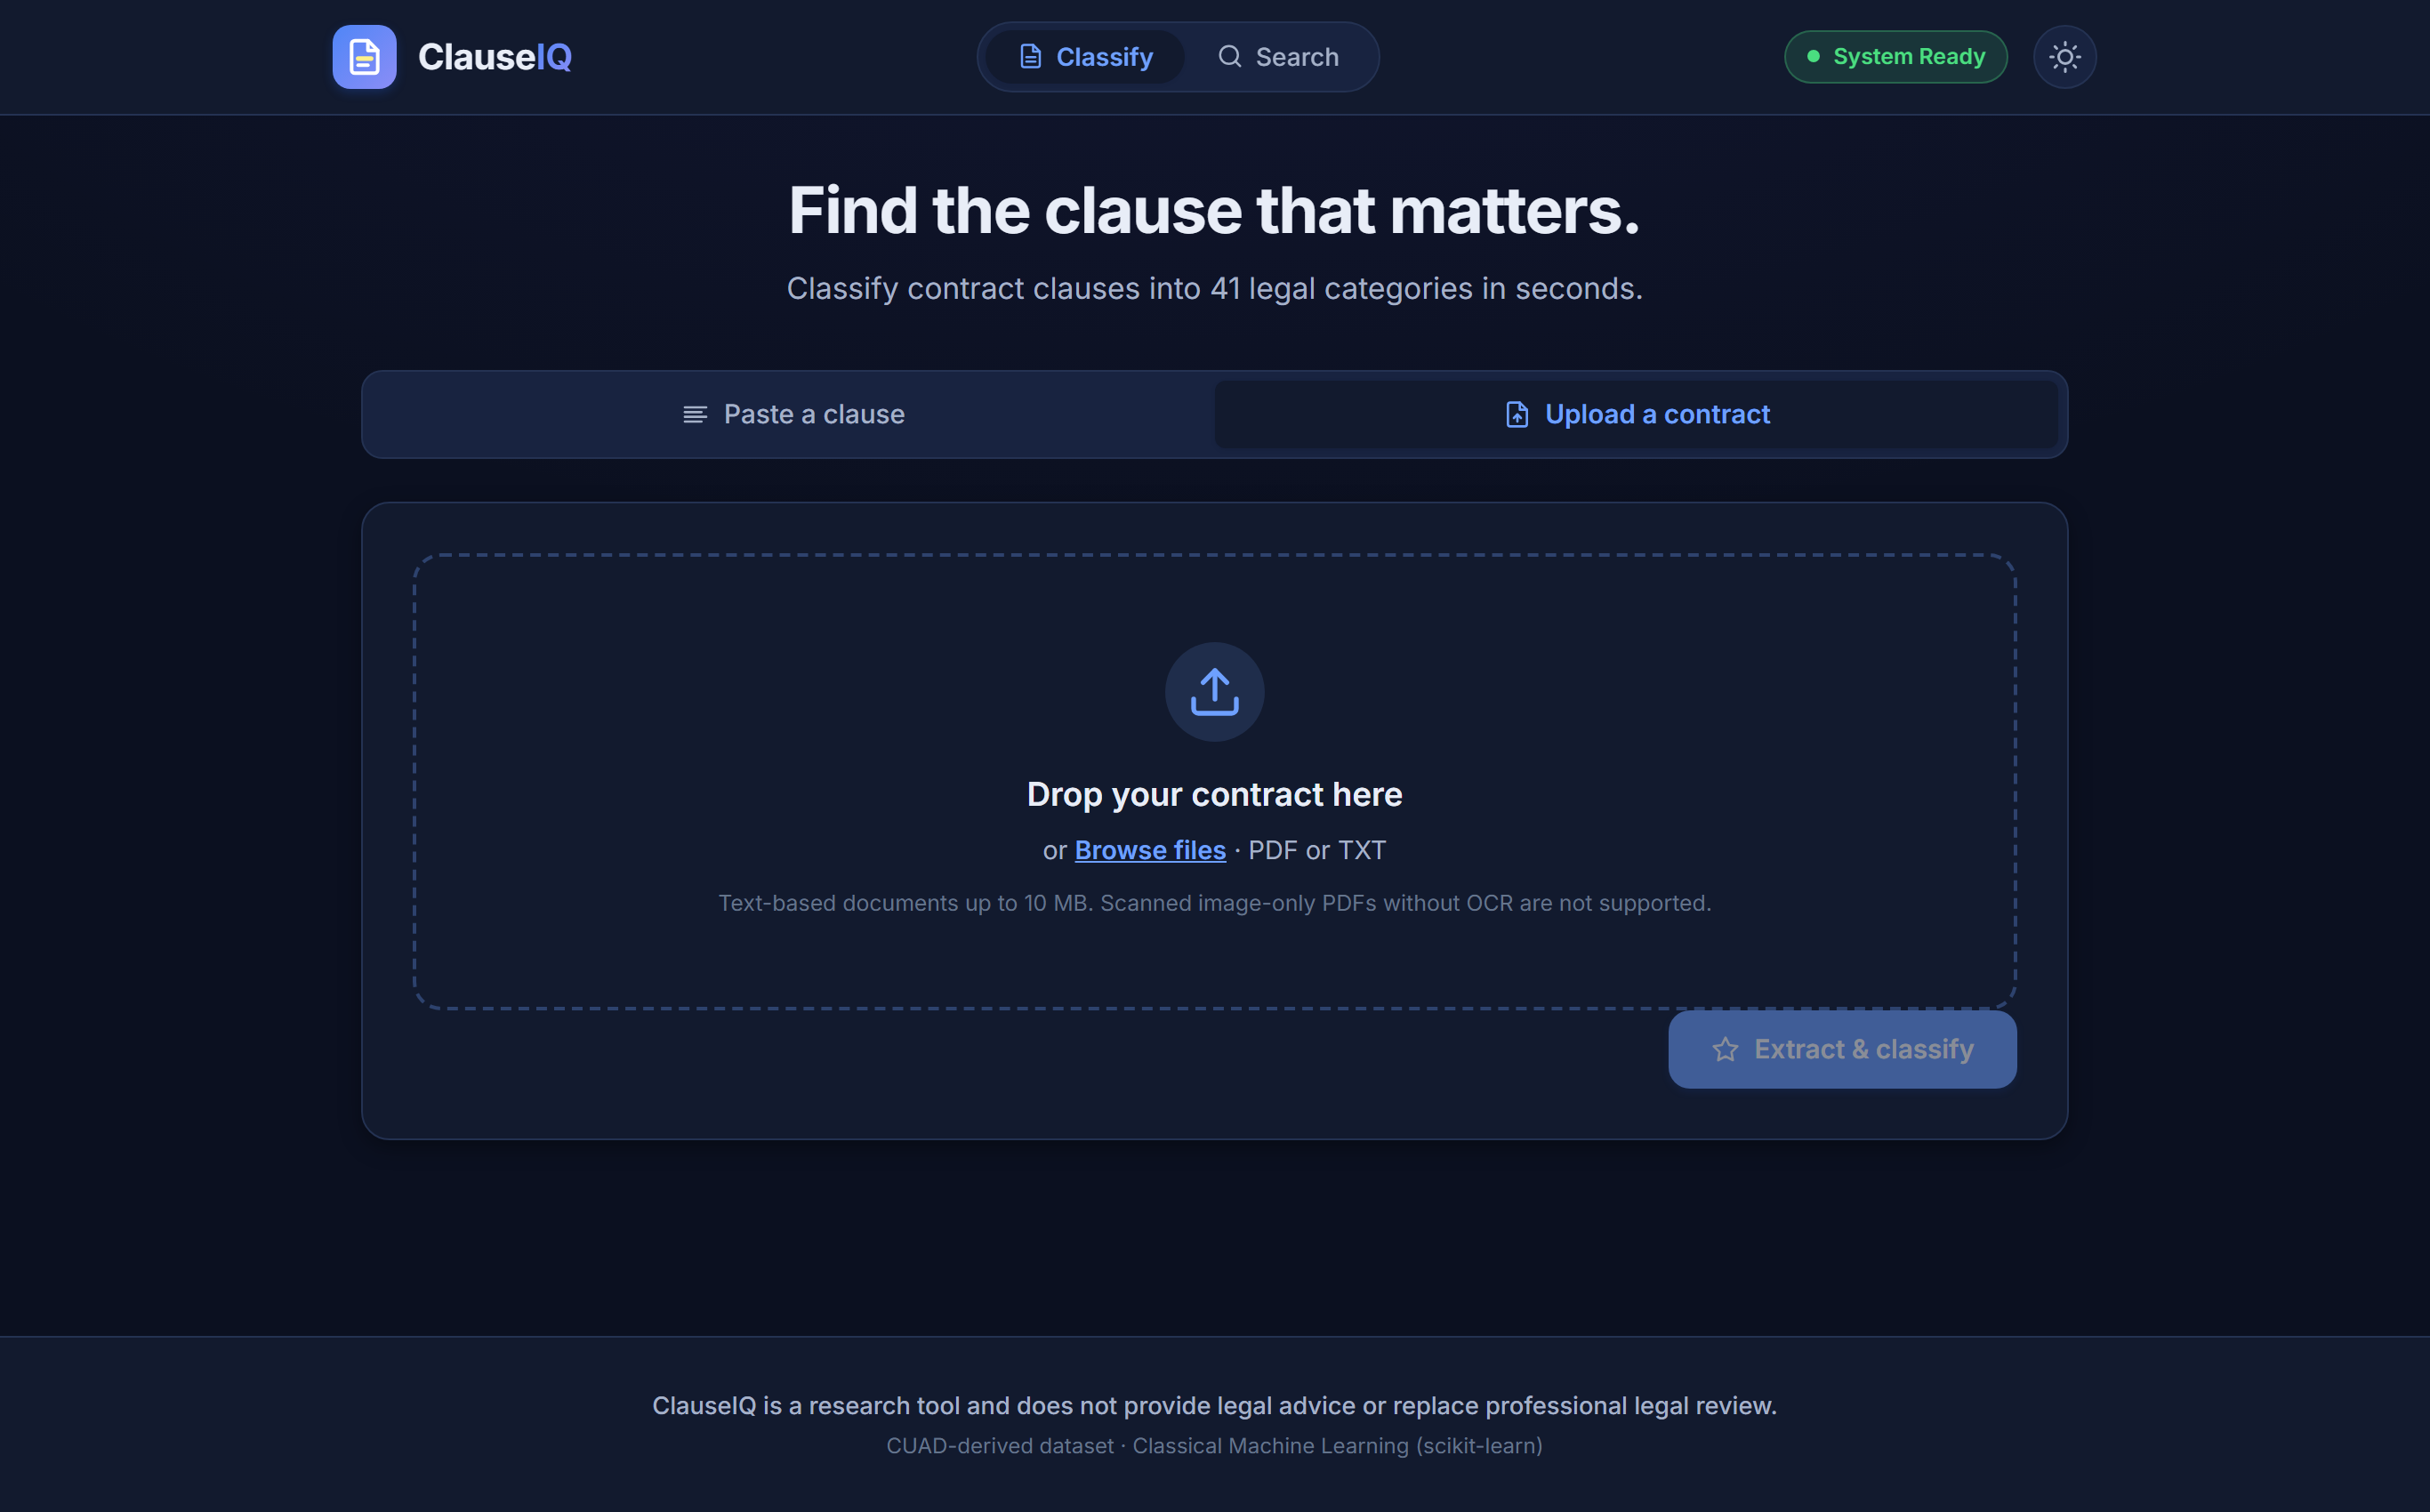
\includegraphics[width=0.88\textwidth]{figures/ui/ui_02_classify_upload_dropzone.png}
\caption{User interface: PDF document upload dropzone with drag-and-drop ingestion support}\label{fig:ui_upload_dropzone}
\end{figure}

Figure~\ref{fig:ui_document_results} displays the extraction and classification results for the test agreement \path{sample_contract.pdf}. The view presents the document status summary (29 extracted clauses, breakdown by confidence tier), interactive category filter pills, text search within results, and paginated clause cards.

\begin{figure}[htbp]
\centering
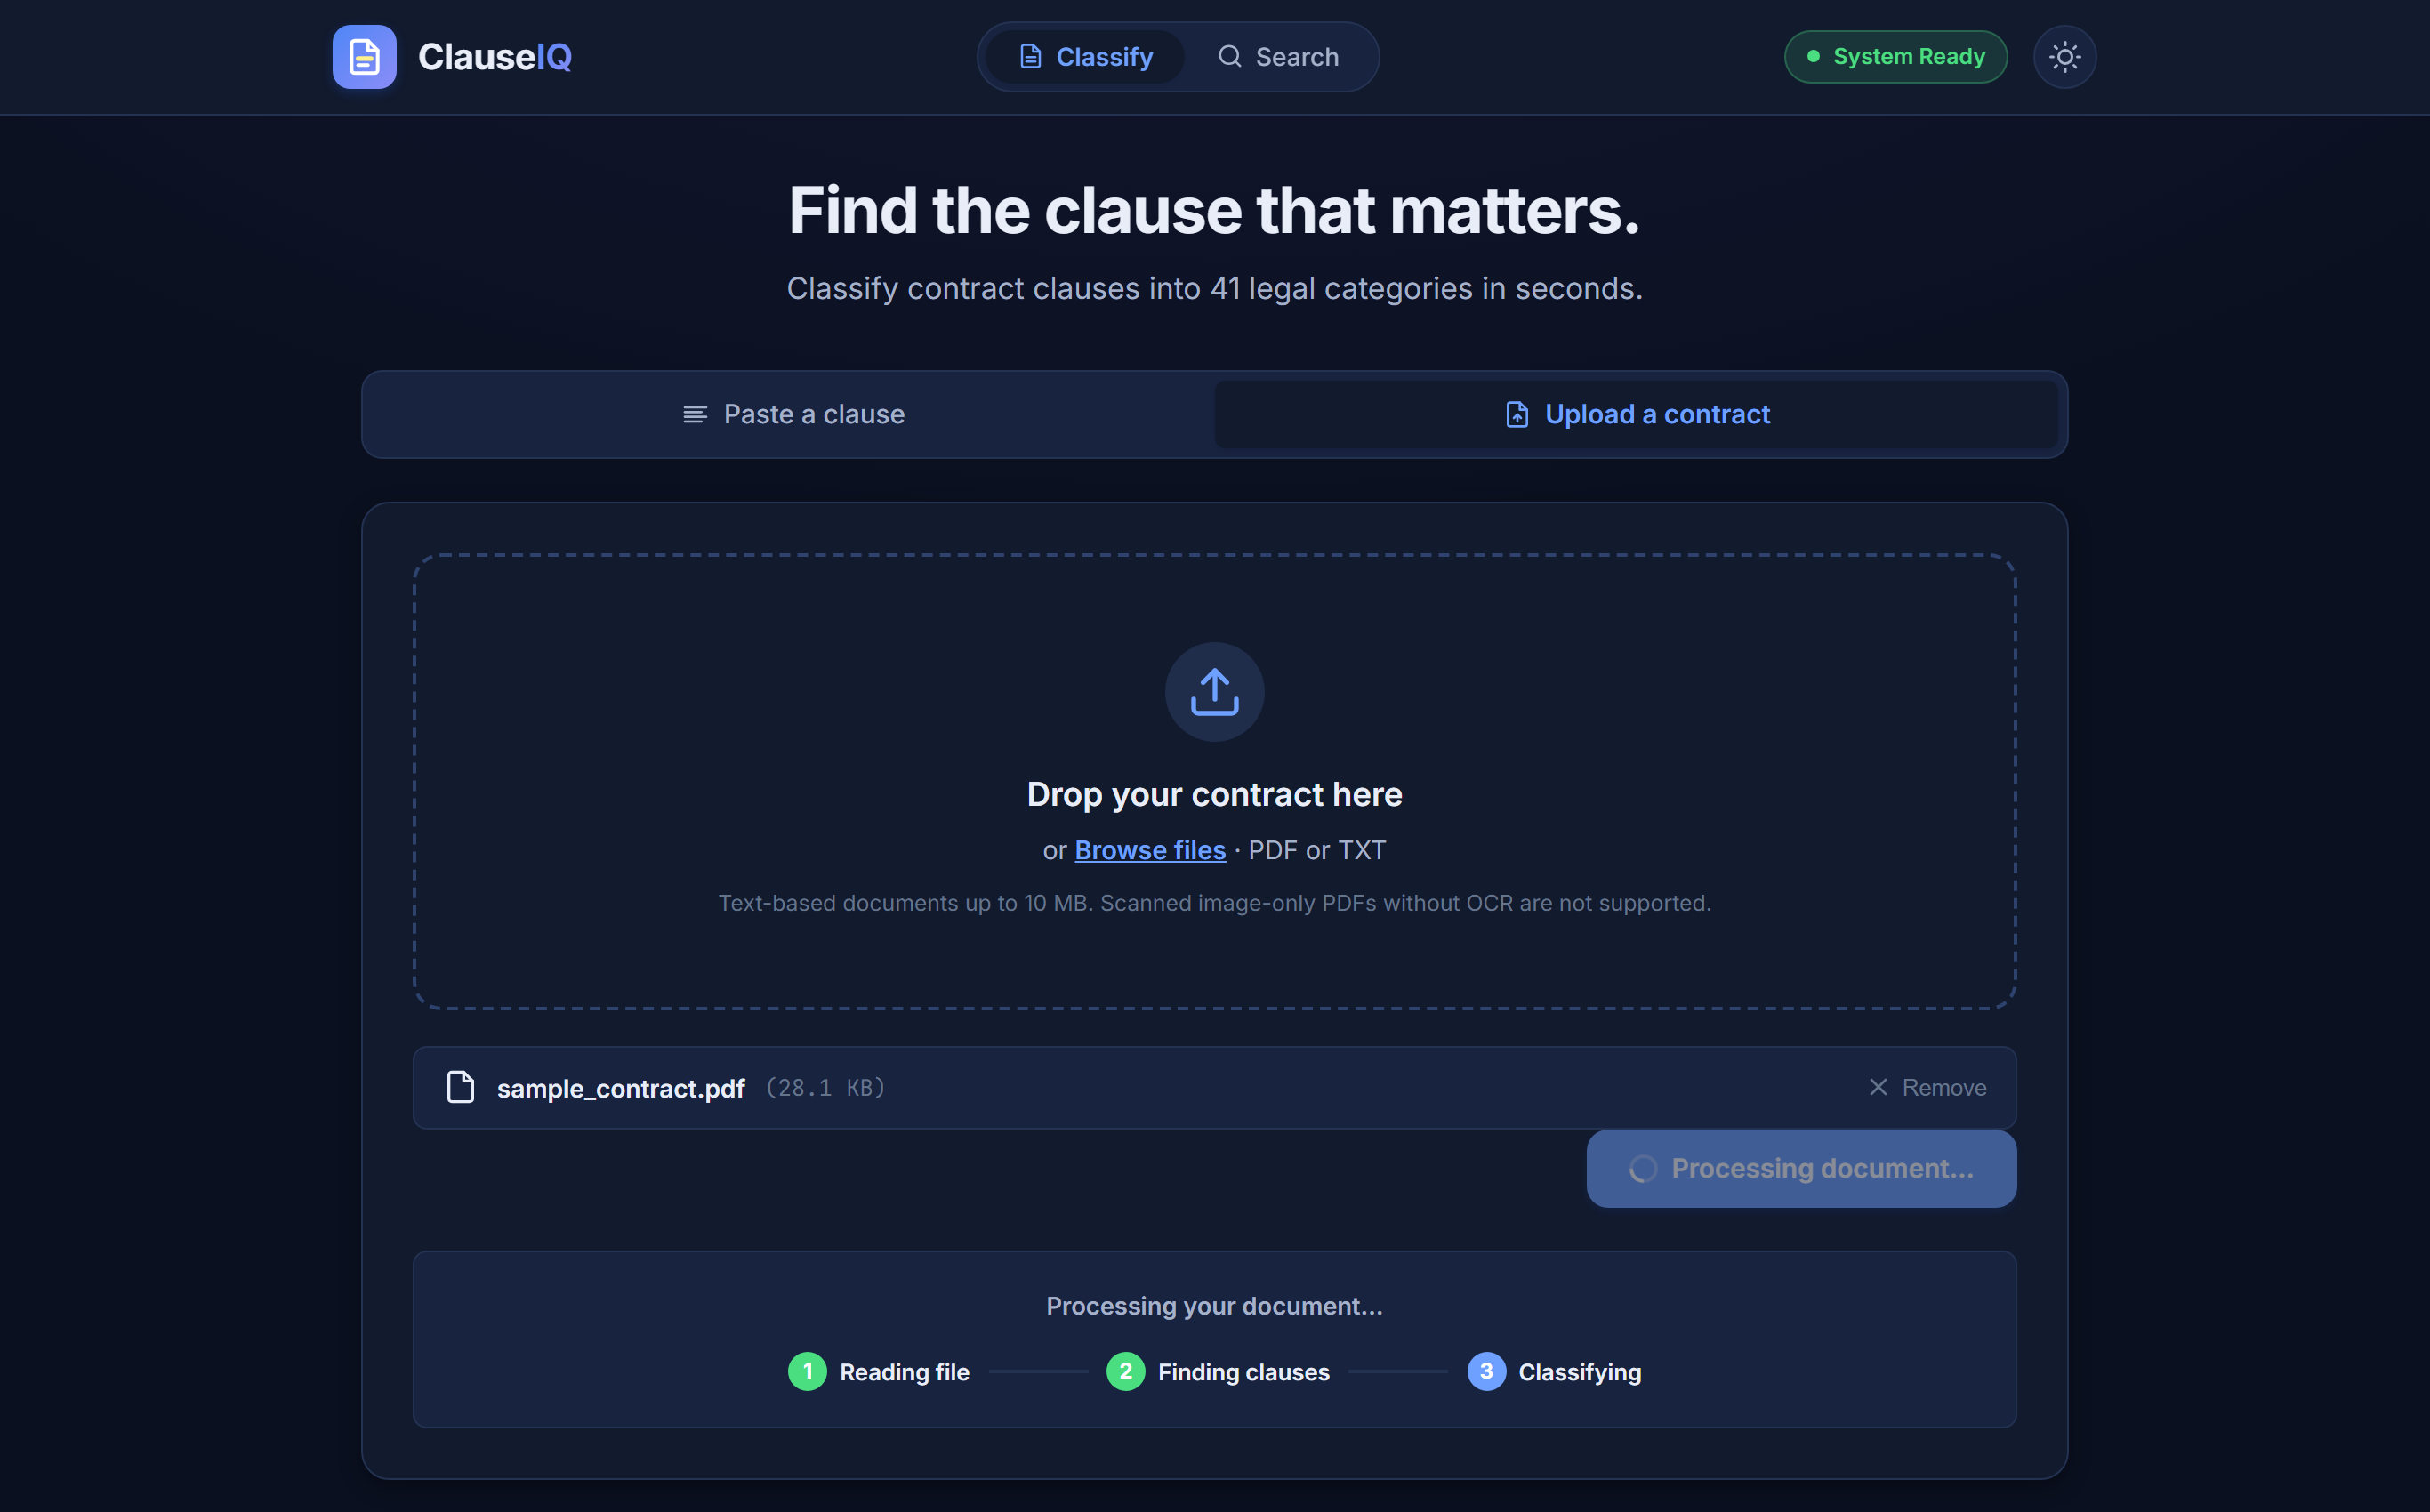
\includegraphics[width=0.88\textwidth]{figures/ui/ui_03_classify_document_results.png}
\caption{User interface: Multi-clause document extraction results table with triage breakdown and filters}\label{fig:ui_document_results}
\end{figure}

Figure~\ref{fig:ui_search_results} illustrates the Intelligent Search interface executing a semantic query (\textit{``limitation of liability for indirect or consequential damages''}) with a \textit{Cap On Liability} category filter. The top ranked clauses are displayed with computed similarity scores and highlighted matching terms.

\begin{figure}[htbp]
\centering
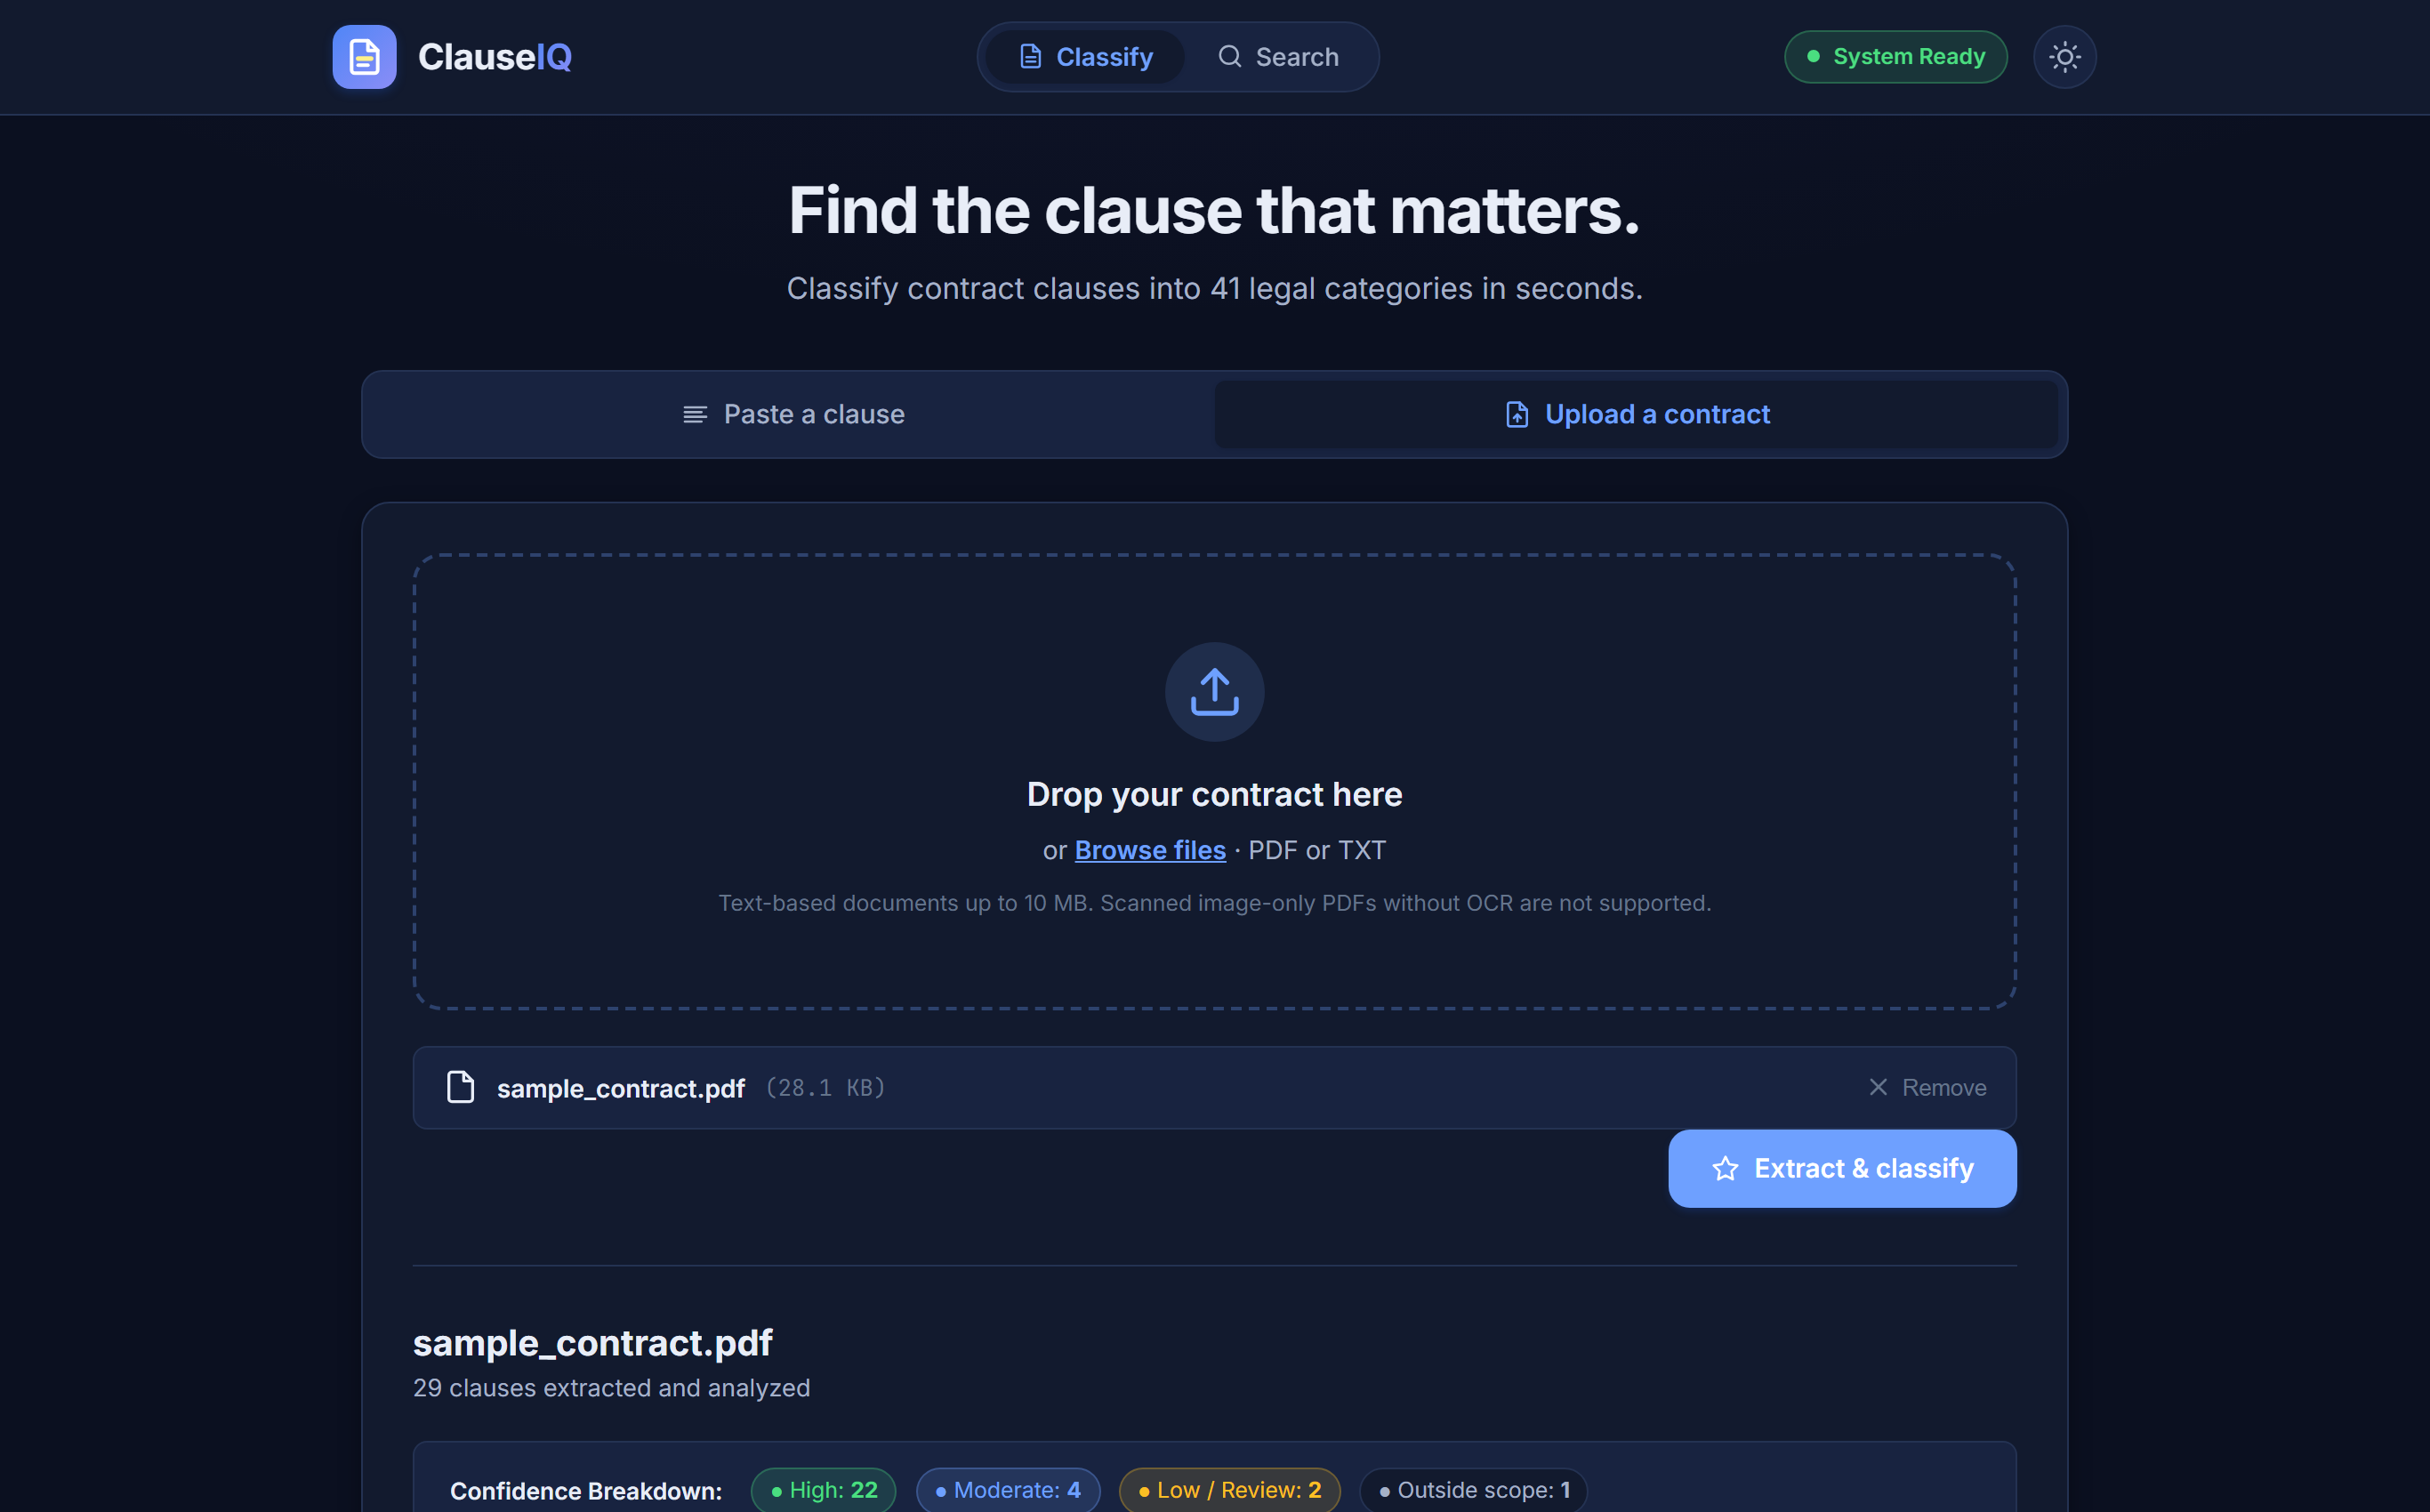
\includegraphics[width=0.88\textwidth]{figures/ui/ui_04_search_results.png}
\caption{User interface: Intelligent semantic search console with category filter and highlighted terms}\label{fig:ui_search_results}
\end{figure}

Figure~\ref{fig:ui_dark_mode} depicts the full application rendered in dark mode. The color palette utilizes curated dark tokens with high text contrast, designed to reduce ocular fatigue during lengthy document auditing sessions.

\begin{figure}[htbp]
\centering
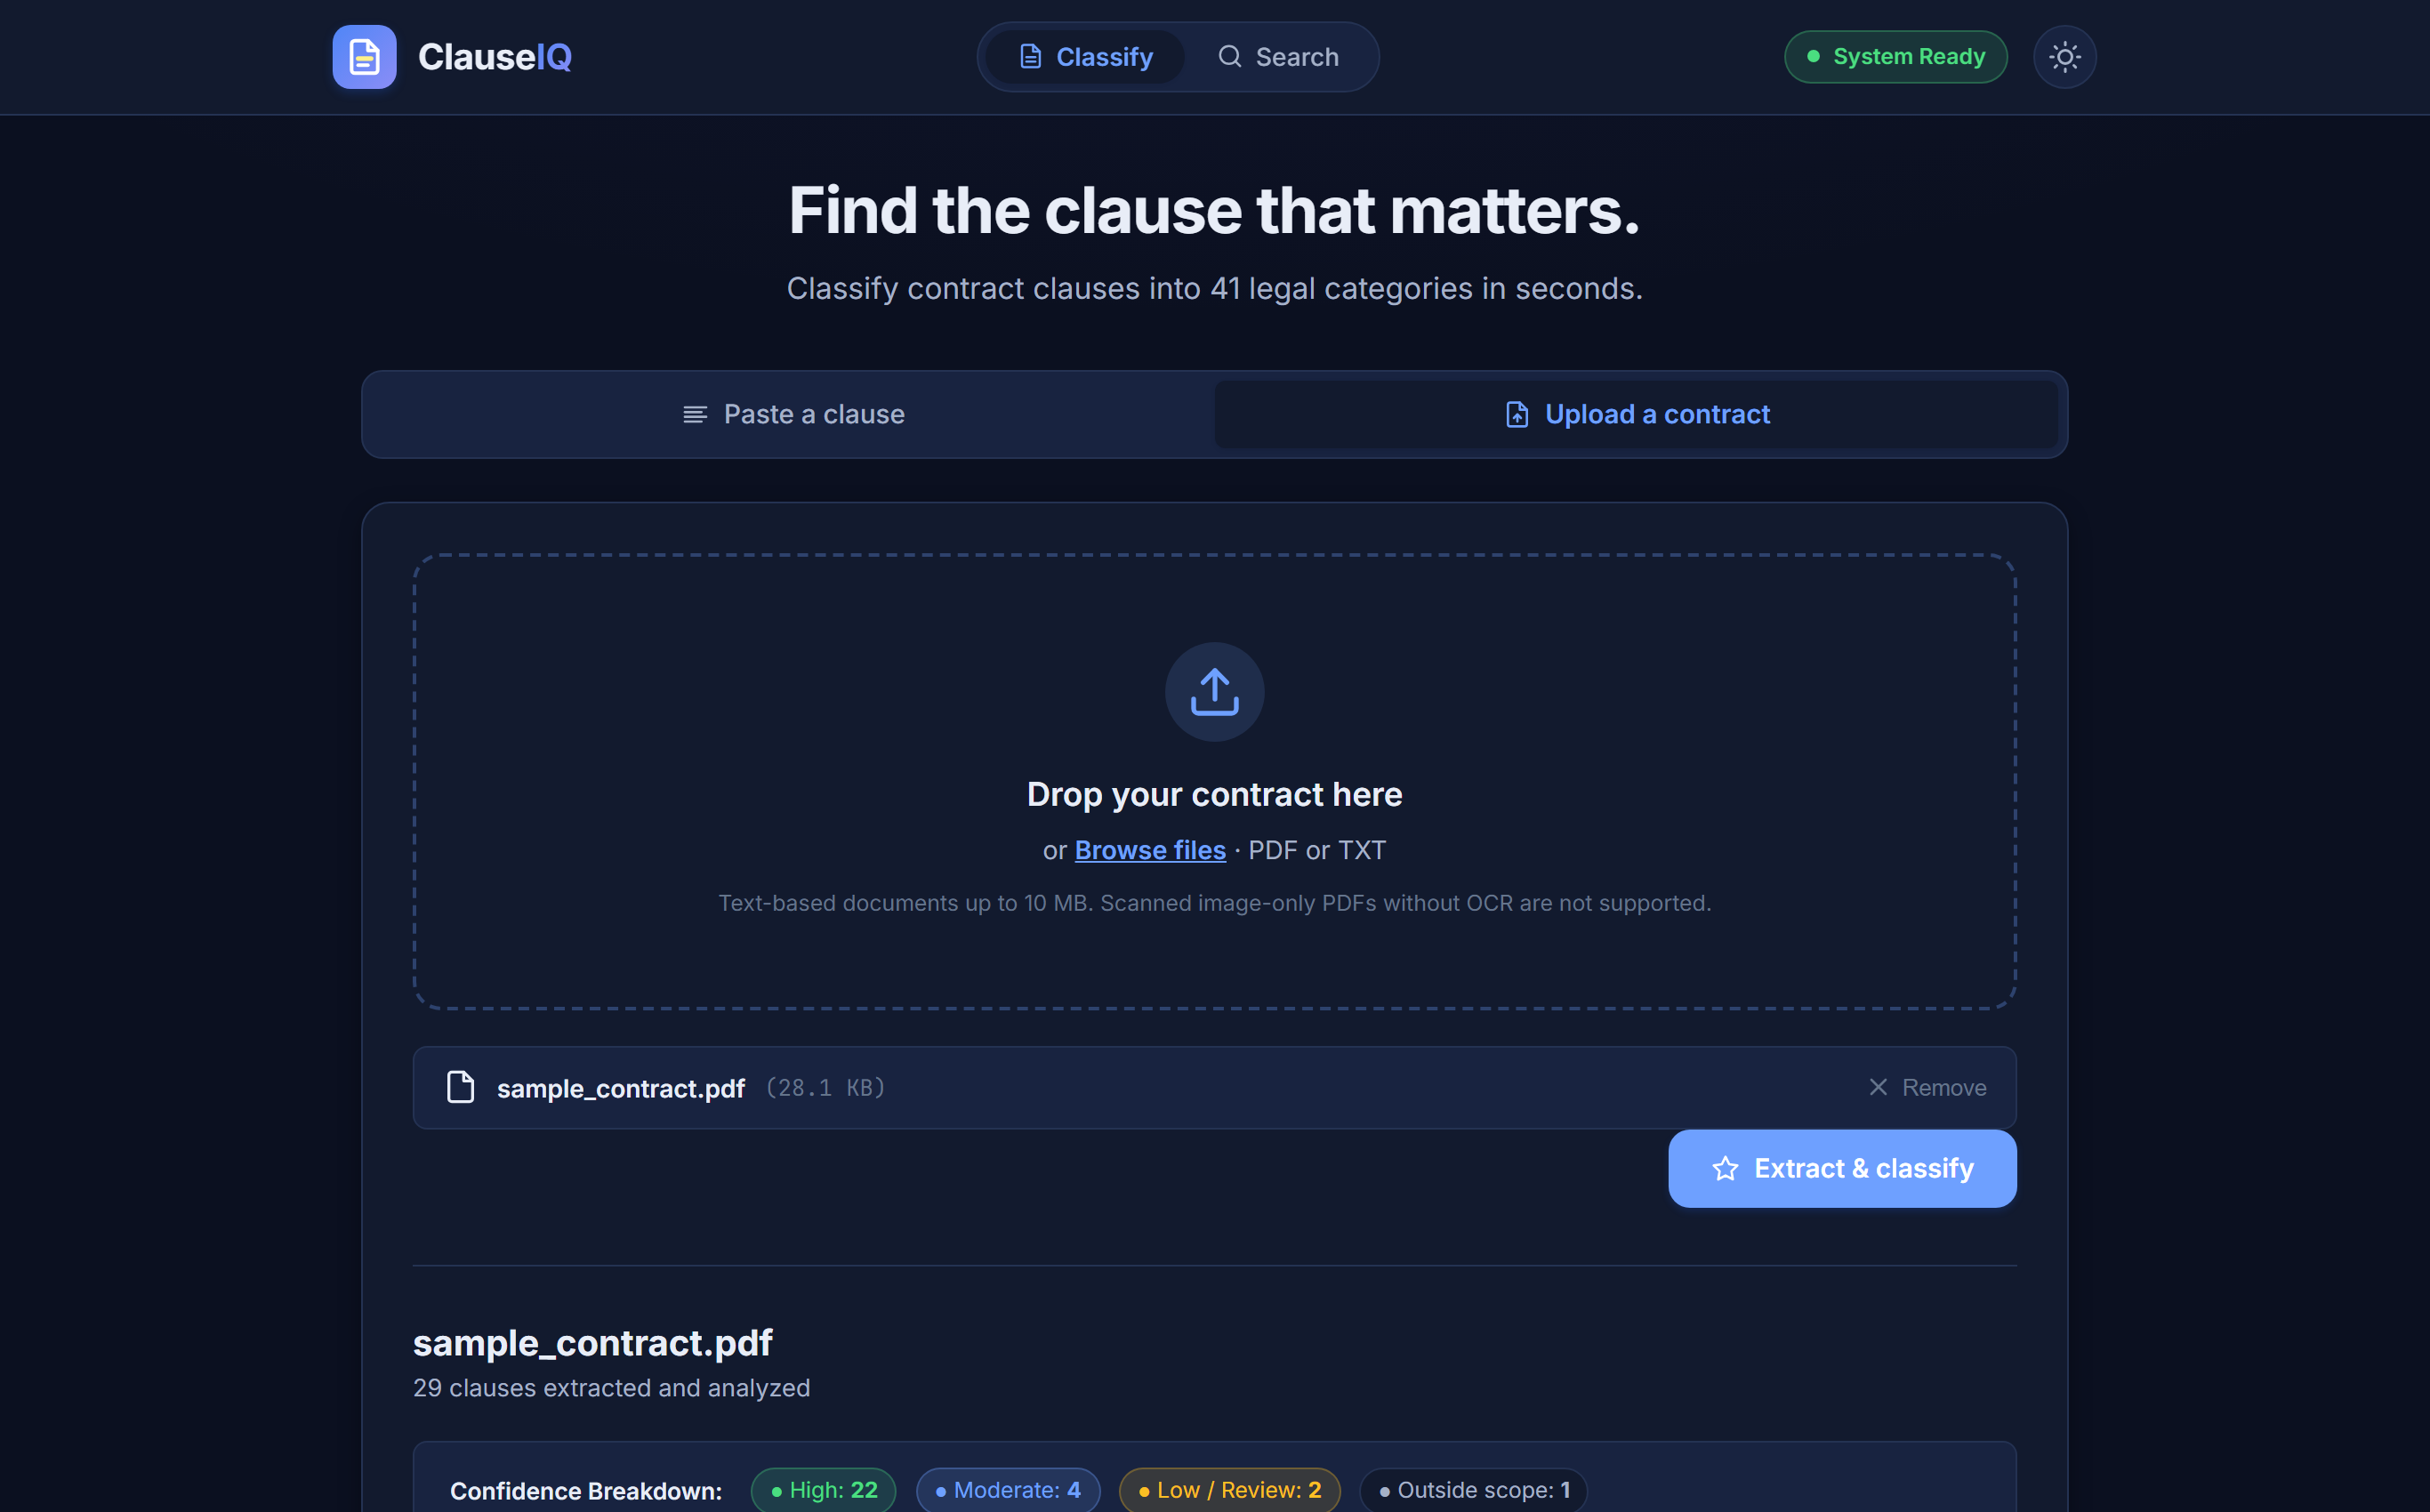
\includegraphics[width=0.88\textwidth]{figures/ui/ui_05_dark_mode.png}
\caption{User interface: Dark mode theme aesthetic optimized for extended review sessions}\label{fig:ui_dark_mode}
\end{figure}

Figure~\ref{fig:ui_mobile_view} captures the application on a mobile viewport (390~px width). The layout adapts responsively, stacking input controls vertically, scaling fonts, and rendering a convenient bottom navigation bar for view switching.

\begin{figure}[htbp]
\centering
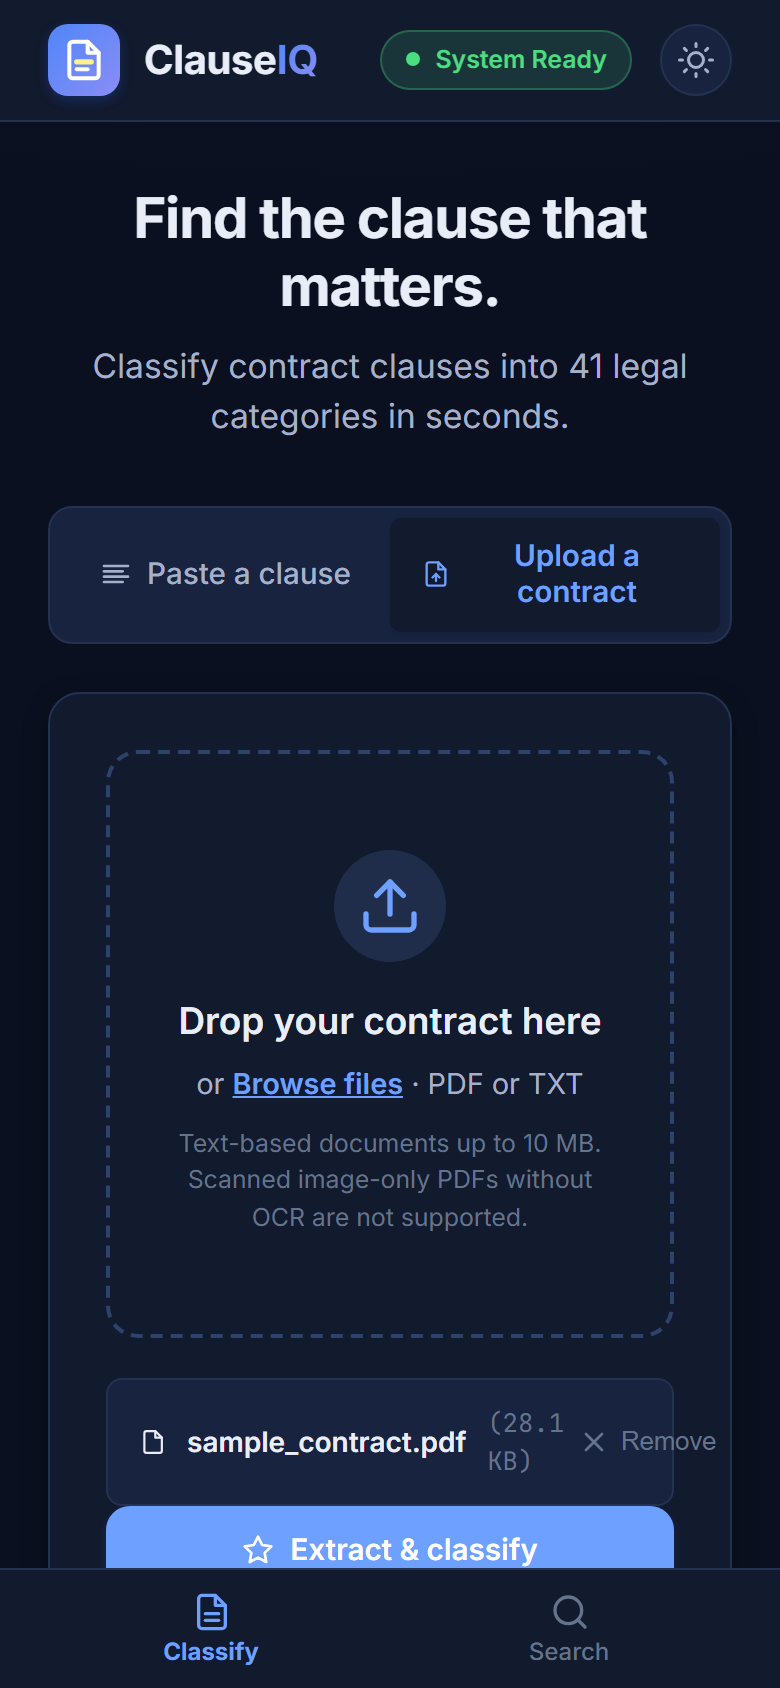
\includegraphics[width=0.55\textwidth]{figures/ui/ui_06_mobile_view.png}
\caption{User interface: Responsive mobile layout (390 px width) with mobile bottom navigation bar}\label{fig:ui_mobile_view}
\end{figure}

Figure~\ref{fig:ui_offline_banner} demonstrates system fault tolerance when the backend server is stopped. The \texttt{OfflineBanner} appears at the top of the viewport in amber, notifying the user that the backend is offline and that classification actions are temporarily paused.

\begin{figure}[htbp]
\centering
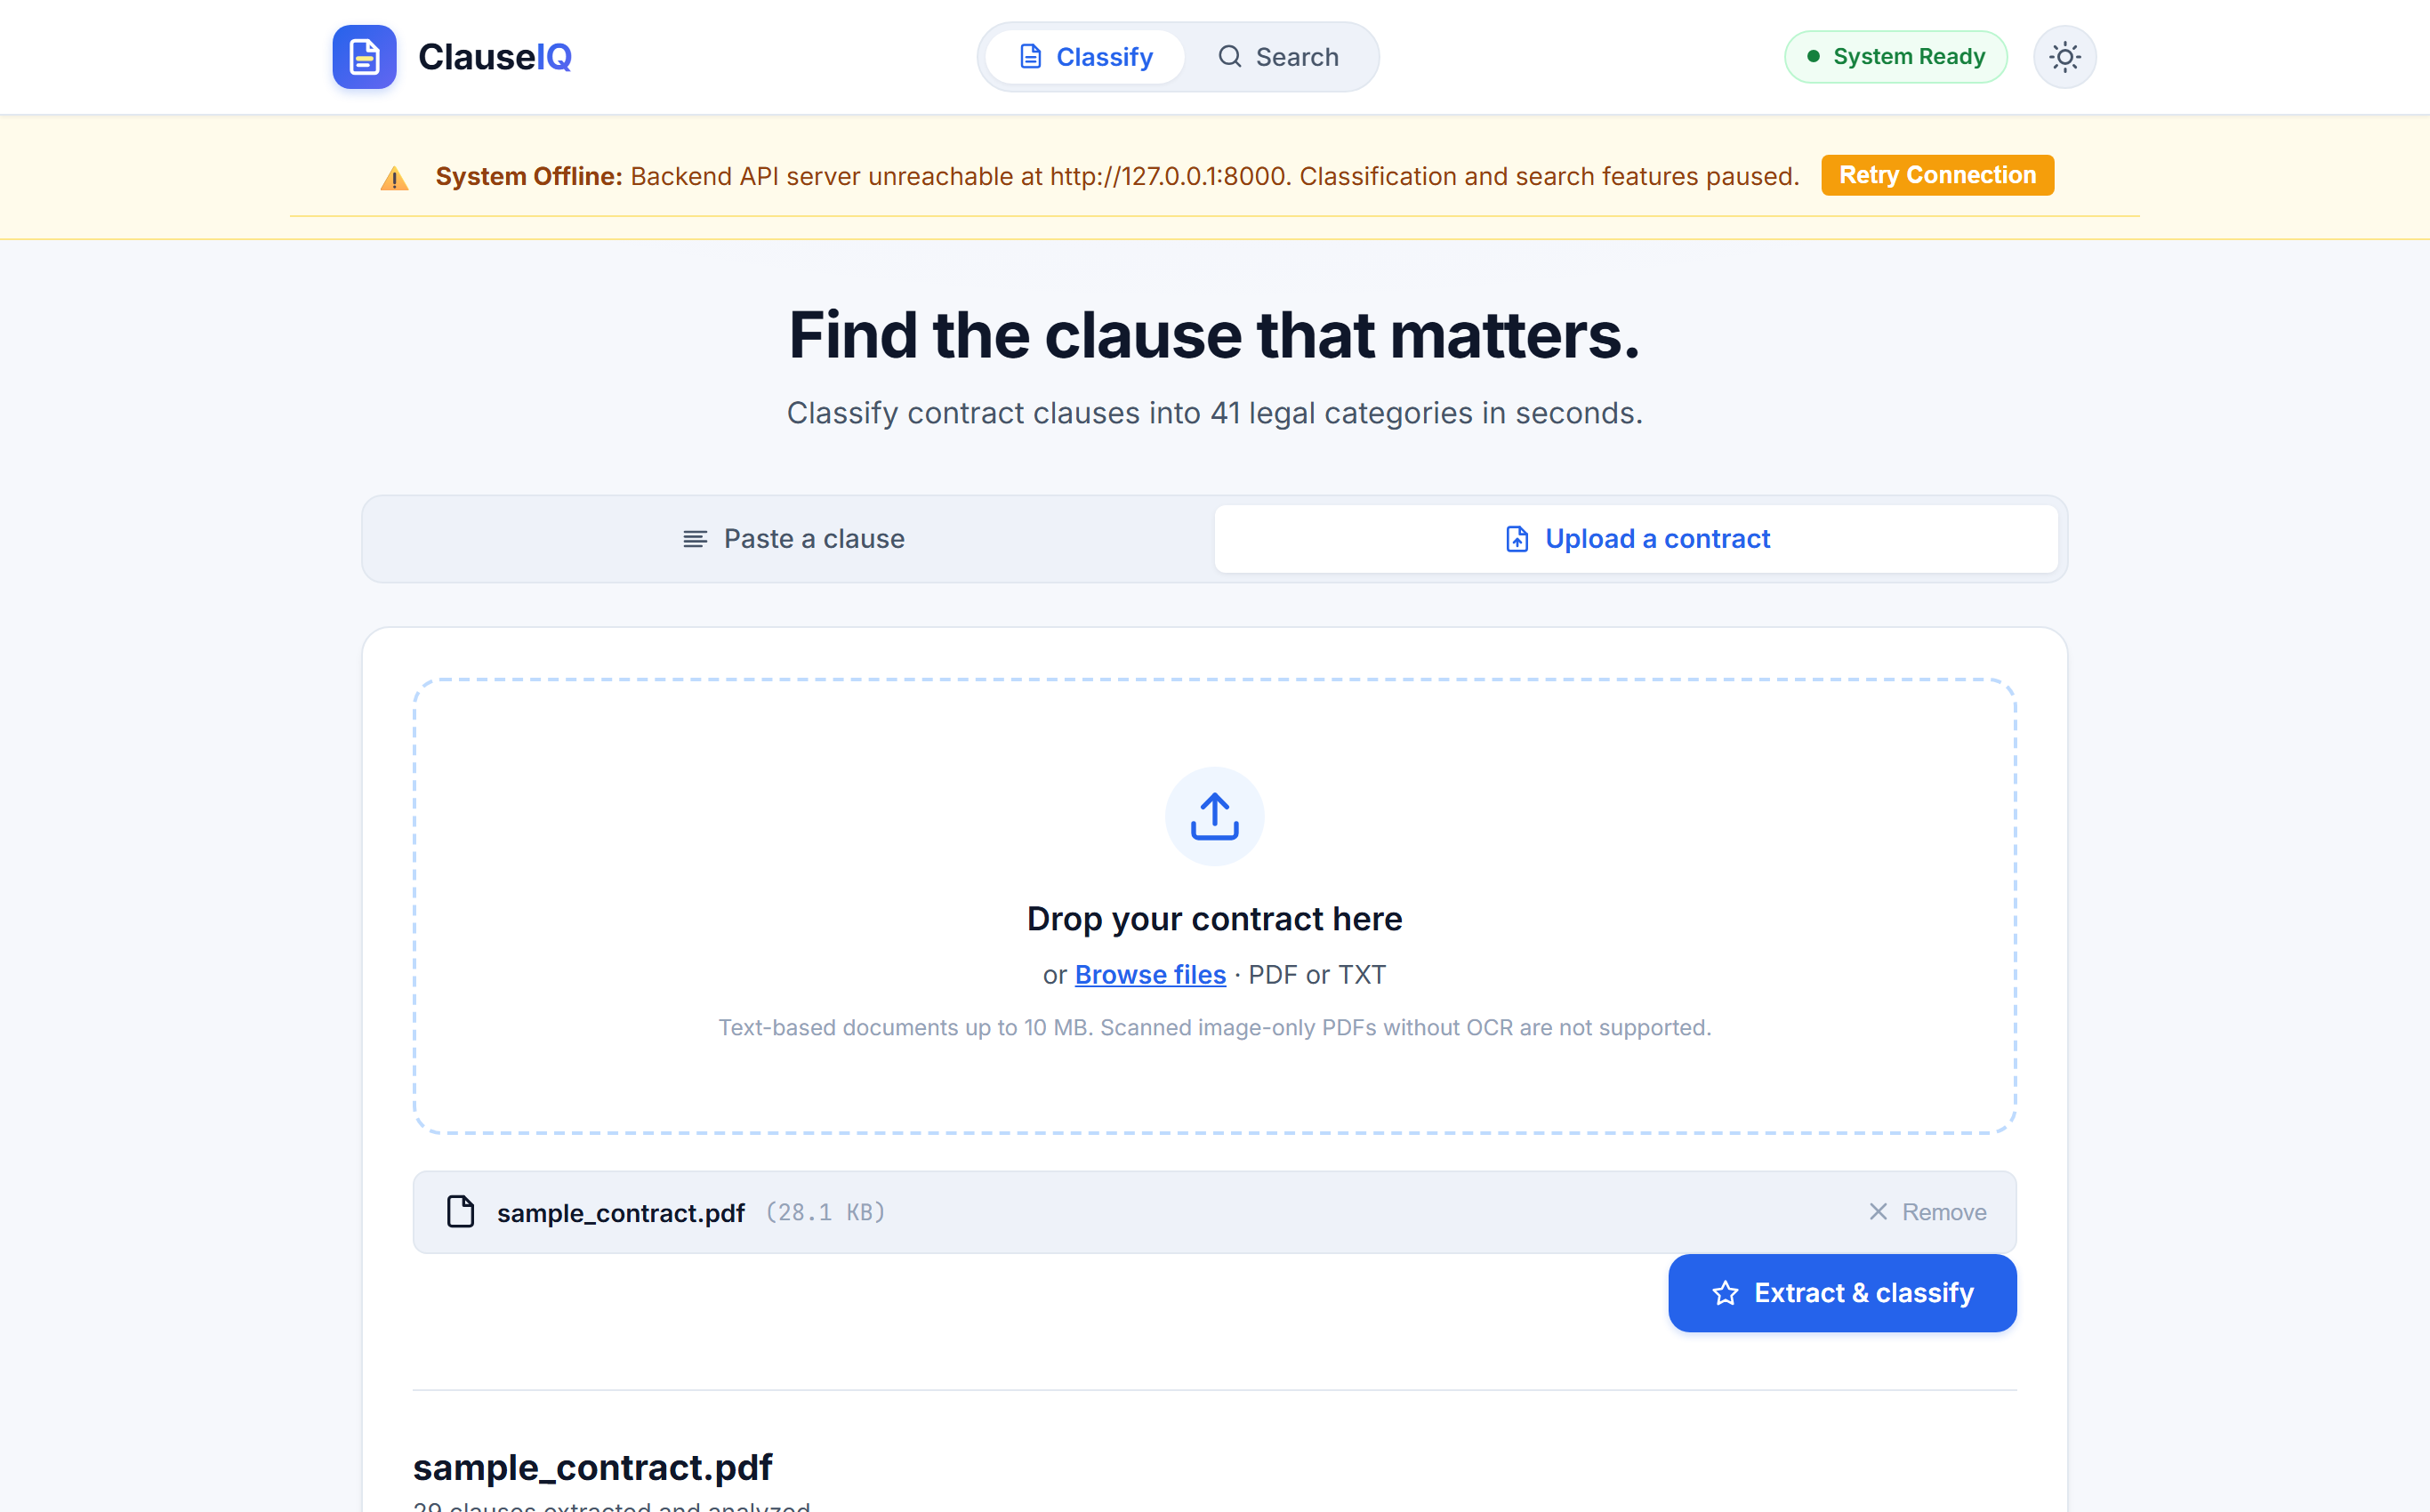
\includegraphics[width=0.88\textwidth]{figures/ui/ui_07_offline_banner.png}
\caption{User interface: Offline banner alerting the user when the backend API service is disconnected}\label{fig:ui_offline_banner}
\end{figure}

Figure~\ref{fig:ui_api_docs} displays the interactive FastAPI OpenAPI documentation interface accessible at \texttt{/docs}. The Swagger UI provides an interactive specification of all seven backend endpoints, including schemas and interactive trial calls.

\begin{figure}[!htbp]
\centering
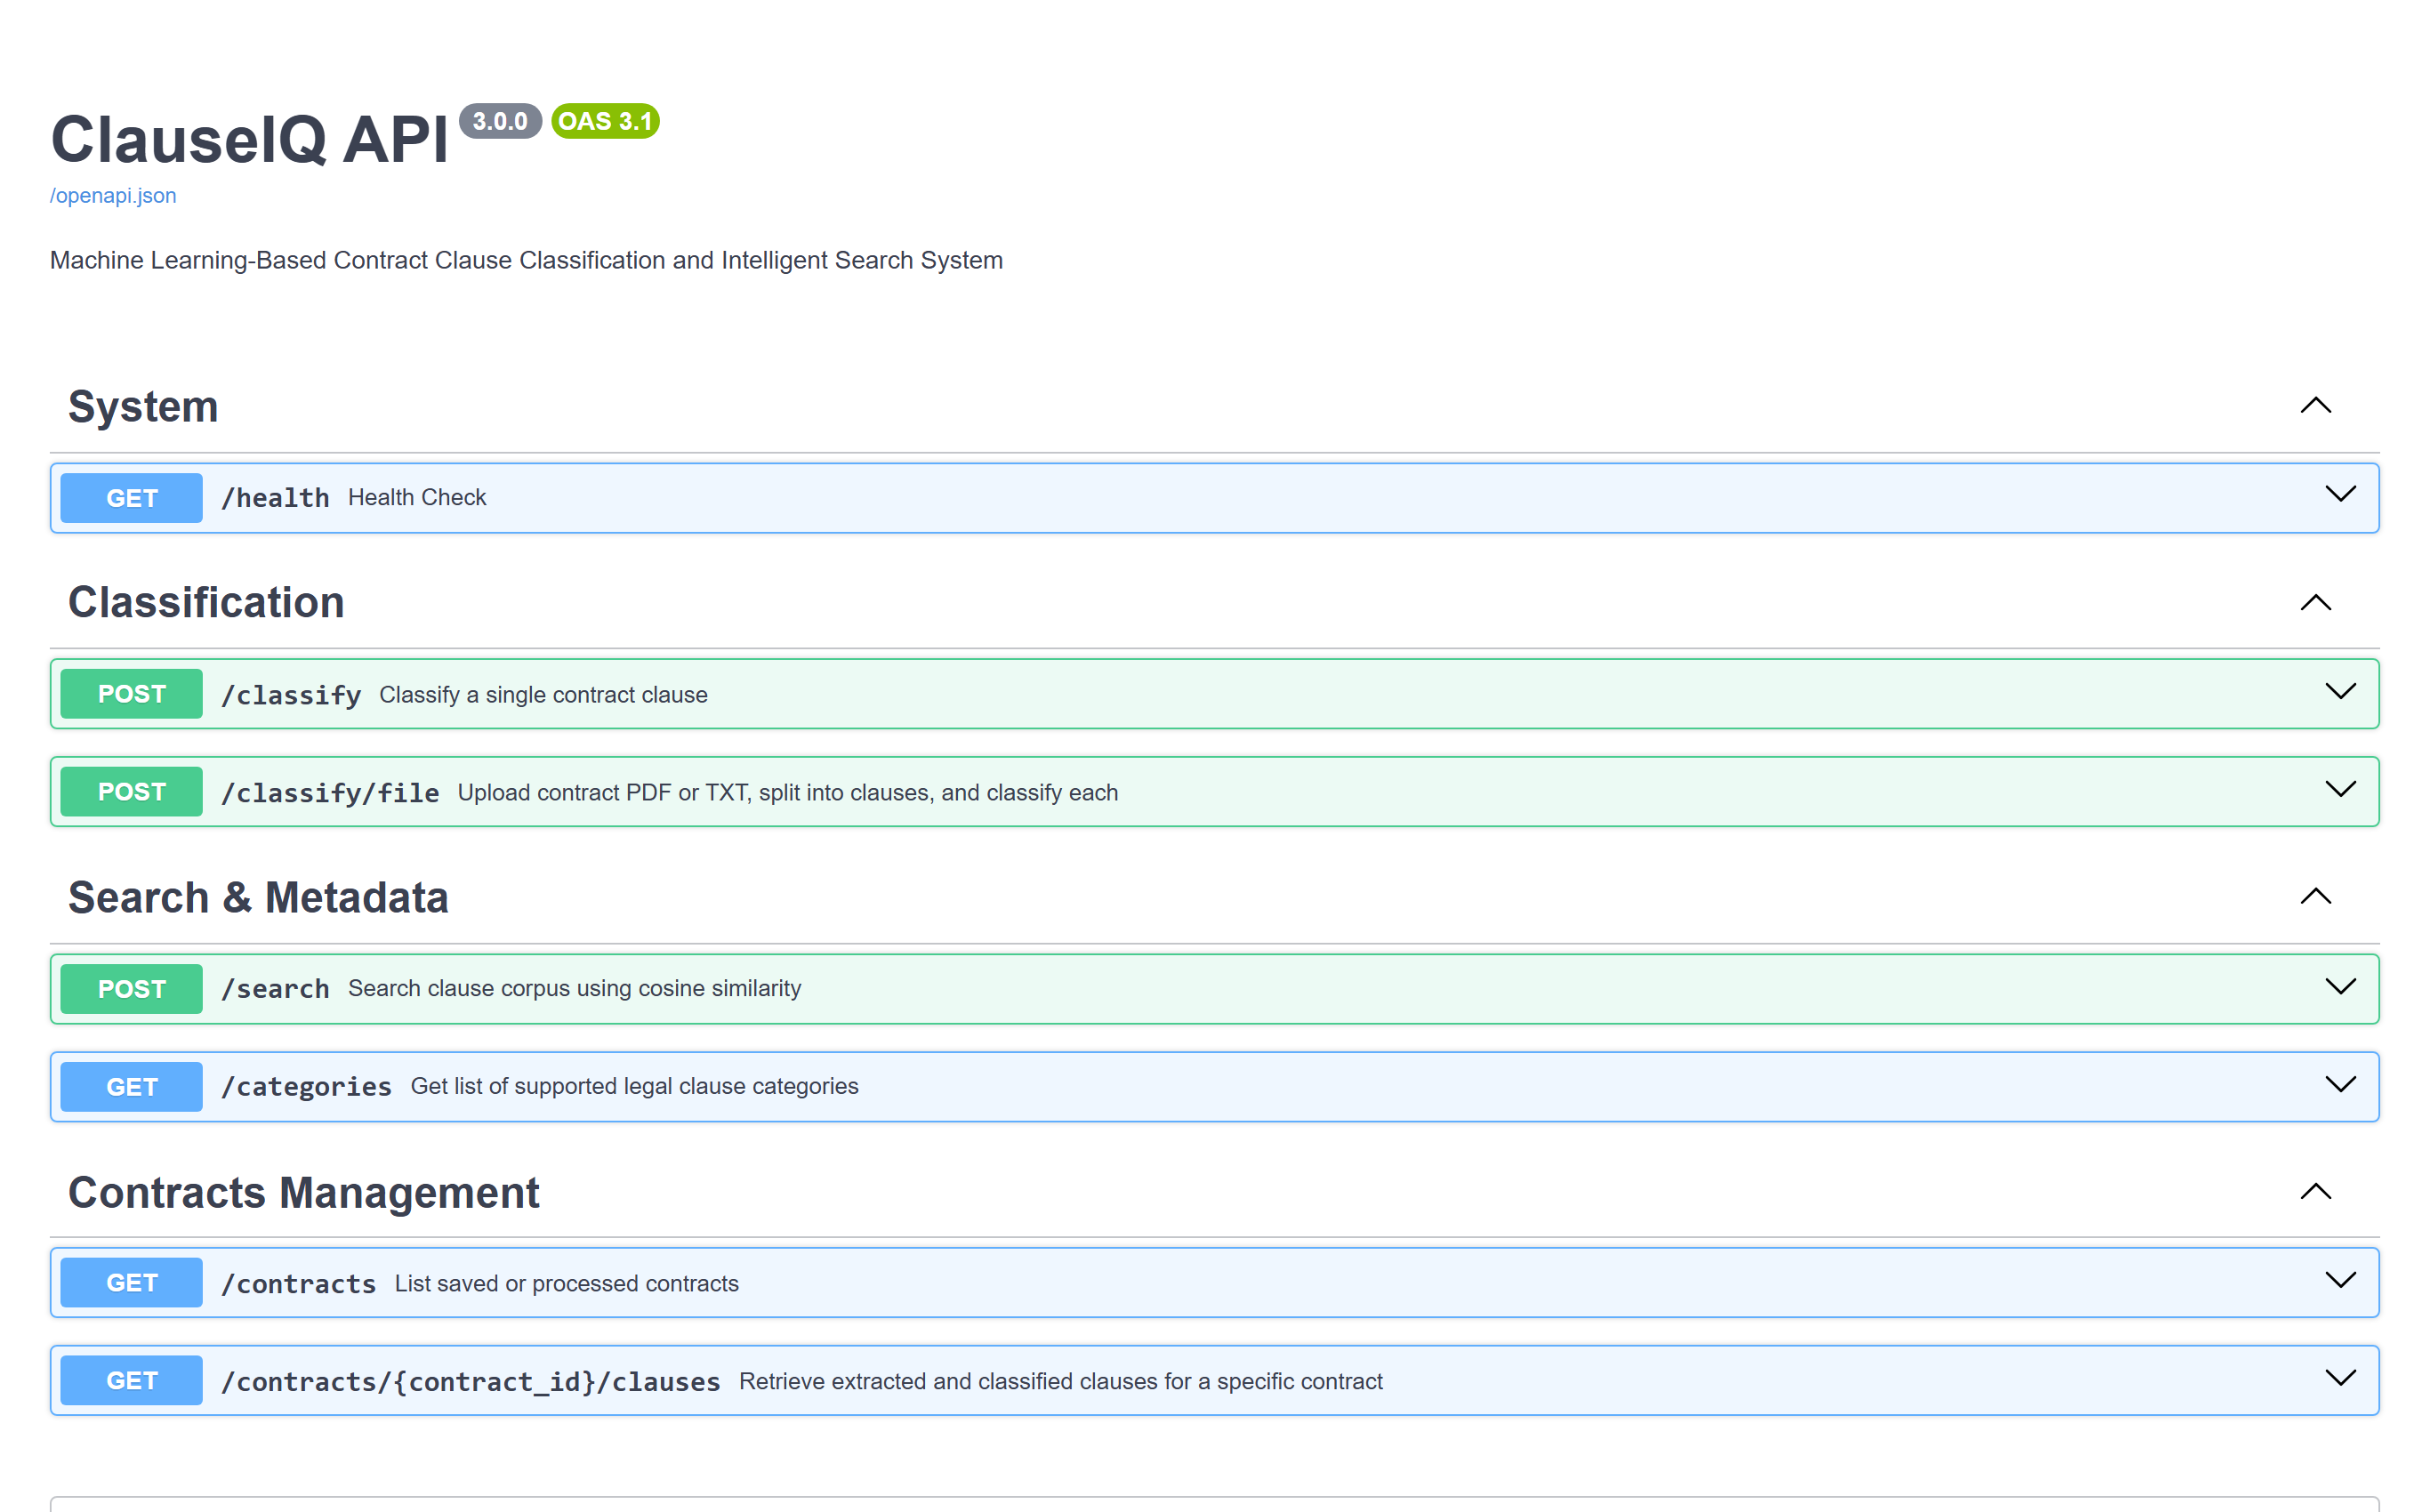
\includegraphics[width=0.80\textwidth]{figures/ui/ui_08_api_docs.png}
\caption{User interface: Interactive FastAPI Swagger documentation (\texttt{/docs}) detailing all REST endpoints}\label{fig:ui_api_docs}
\end{figure}
